\documentclass[11pt]{article}

\usepackage[a4paper,margin=1in]{geometry}
\usepackage{amsmath}
\usepackage{amssymb}
\usepackage{enumitem}
\usepackage{graphicx}
\usepackage{float}

\begin{document}

\begin{center}

{\Large\bfseries
A Workload-Aware Dynamic Array Growth Algorithm for Efficient Memory Allocation
}

\end{center}

\section*{Background}

Dynamic arrays are fundamental structures in modern software for fast random
access and dynamic memory allocation. Conventional implementations resize
arrays using fixed growth factors (e.g., $1.5\times$ or $2\times$),
compromising between memory utilization and resizing overhead \cite{brodnik}.
Although recent studies explore alternative array organizations to improve
memory efficiency \cite{sartor,bille}, their resizing strategies remain
workload-independent, showing limited adaptability. This study proposes an
adaptive growth strategy combining resize iteration history with runtime
workload intensity.

\section*{Method}

The proposed algorithm models the growth factor using a workload-aware,
GP-optimized hybrid framework:
\[
\scalebox{1.08}{$g(k,v,C_{\text{old}}) = \min\left( g_{\max}, \max\left( g_{\min}, 1 + w_A \left( \frac{\alpha_0 + \lambda \ln(1+v)}{\ln(C_{\text{old}} + \beta)} \right) + (1 - w_A) \left( \frac{c_0 + \lambda \ln(1+v)}{k} \right) \right) \right),$}
\]
where $k$ is the resize history, $v = \frac{\Delta N}{\Delta t}$ is velocity,
$C_{\text{old}}$ is capacity, $w_A$ is the logarithmic weight, and $\lambda$ is
the velocity scaling weight. Constants $\alpha_0 = 3.5, \beta = 10, c_0 = 2.0,
g_{\min} = 1.1, g_{\max} = 2.0$ represent system bounds and parameters.
Parameters $w_A$ and $\lambda$ are optimized using Gaussian Process Bayesian
Optimization, yielding $w_A = 0.9955$ and $\lambda = 3.0944$. Benchmarks were
run across 10 repeated trials ($10^4$--$10^7$ insertions over seven patterns),
comparing the strategy against fixed ($1.5\times, 2.0\times$) growth factors
and the CPython list resizing policy.

\section*{Results and Conclusions}

To evaluate performance, we defined a unified objective $J = 0.4W + 0.4C +
0.2T$, combining normalized memory waste ($W$), copies ($C$), and time ($T$) to
balance spatial and temporal efficiency. Figure \ref{fig:memory_waste} compares
memory waste across evaluated resizing strategies. Under a $10^7$ element mixed
workload, the proposed strategy achieved 0.42\% memory waste, 20 resizes,
10.49M copied elements, and a J-score of 0.2589. Comparatively, Fixed
2.0$\times$ yielded 4.63\% waste (20 resizes, 10.49M copies, $J=0.64$), Fixed
1.5$\times$ yielded 27.77\% waste (35 resizes, 27.69M copies, $J=2.75$), and
Python list yielded 4.59\% waste (102 resizes, 83.84M copies, $J=0.95$). This
represents a 90.9\% memory waste reduction relative to Fixed 2.0$\times$
without increasing resizes or copies under this pattern. Across workloads, the
strategy dynamically adjusted growth to restrict memory waste while keeping
resizing overhead low, contributing a workload-sensitive mechanism.

\begin{figure}[H]
\centering
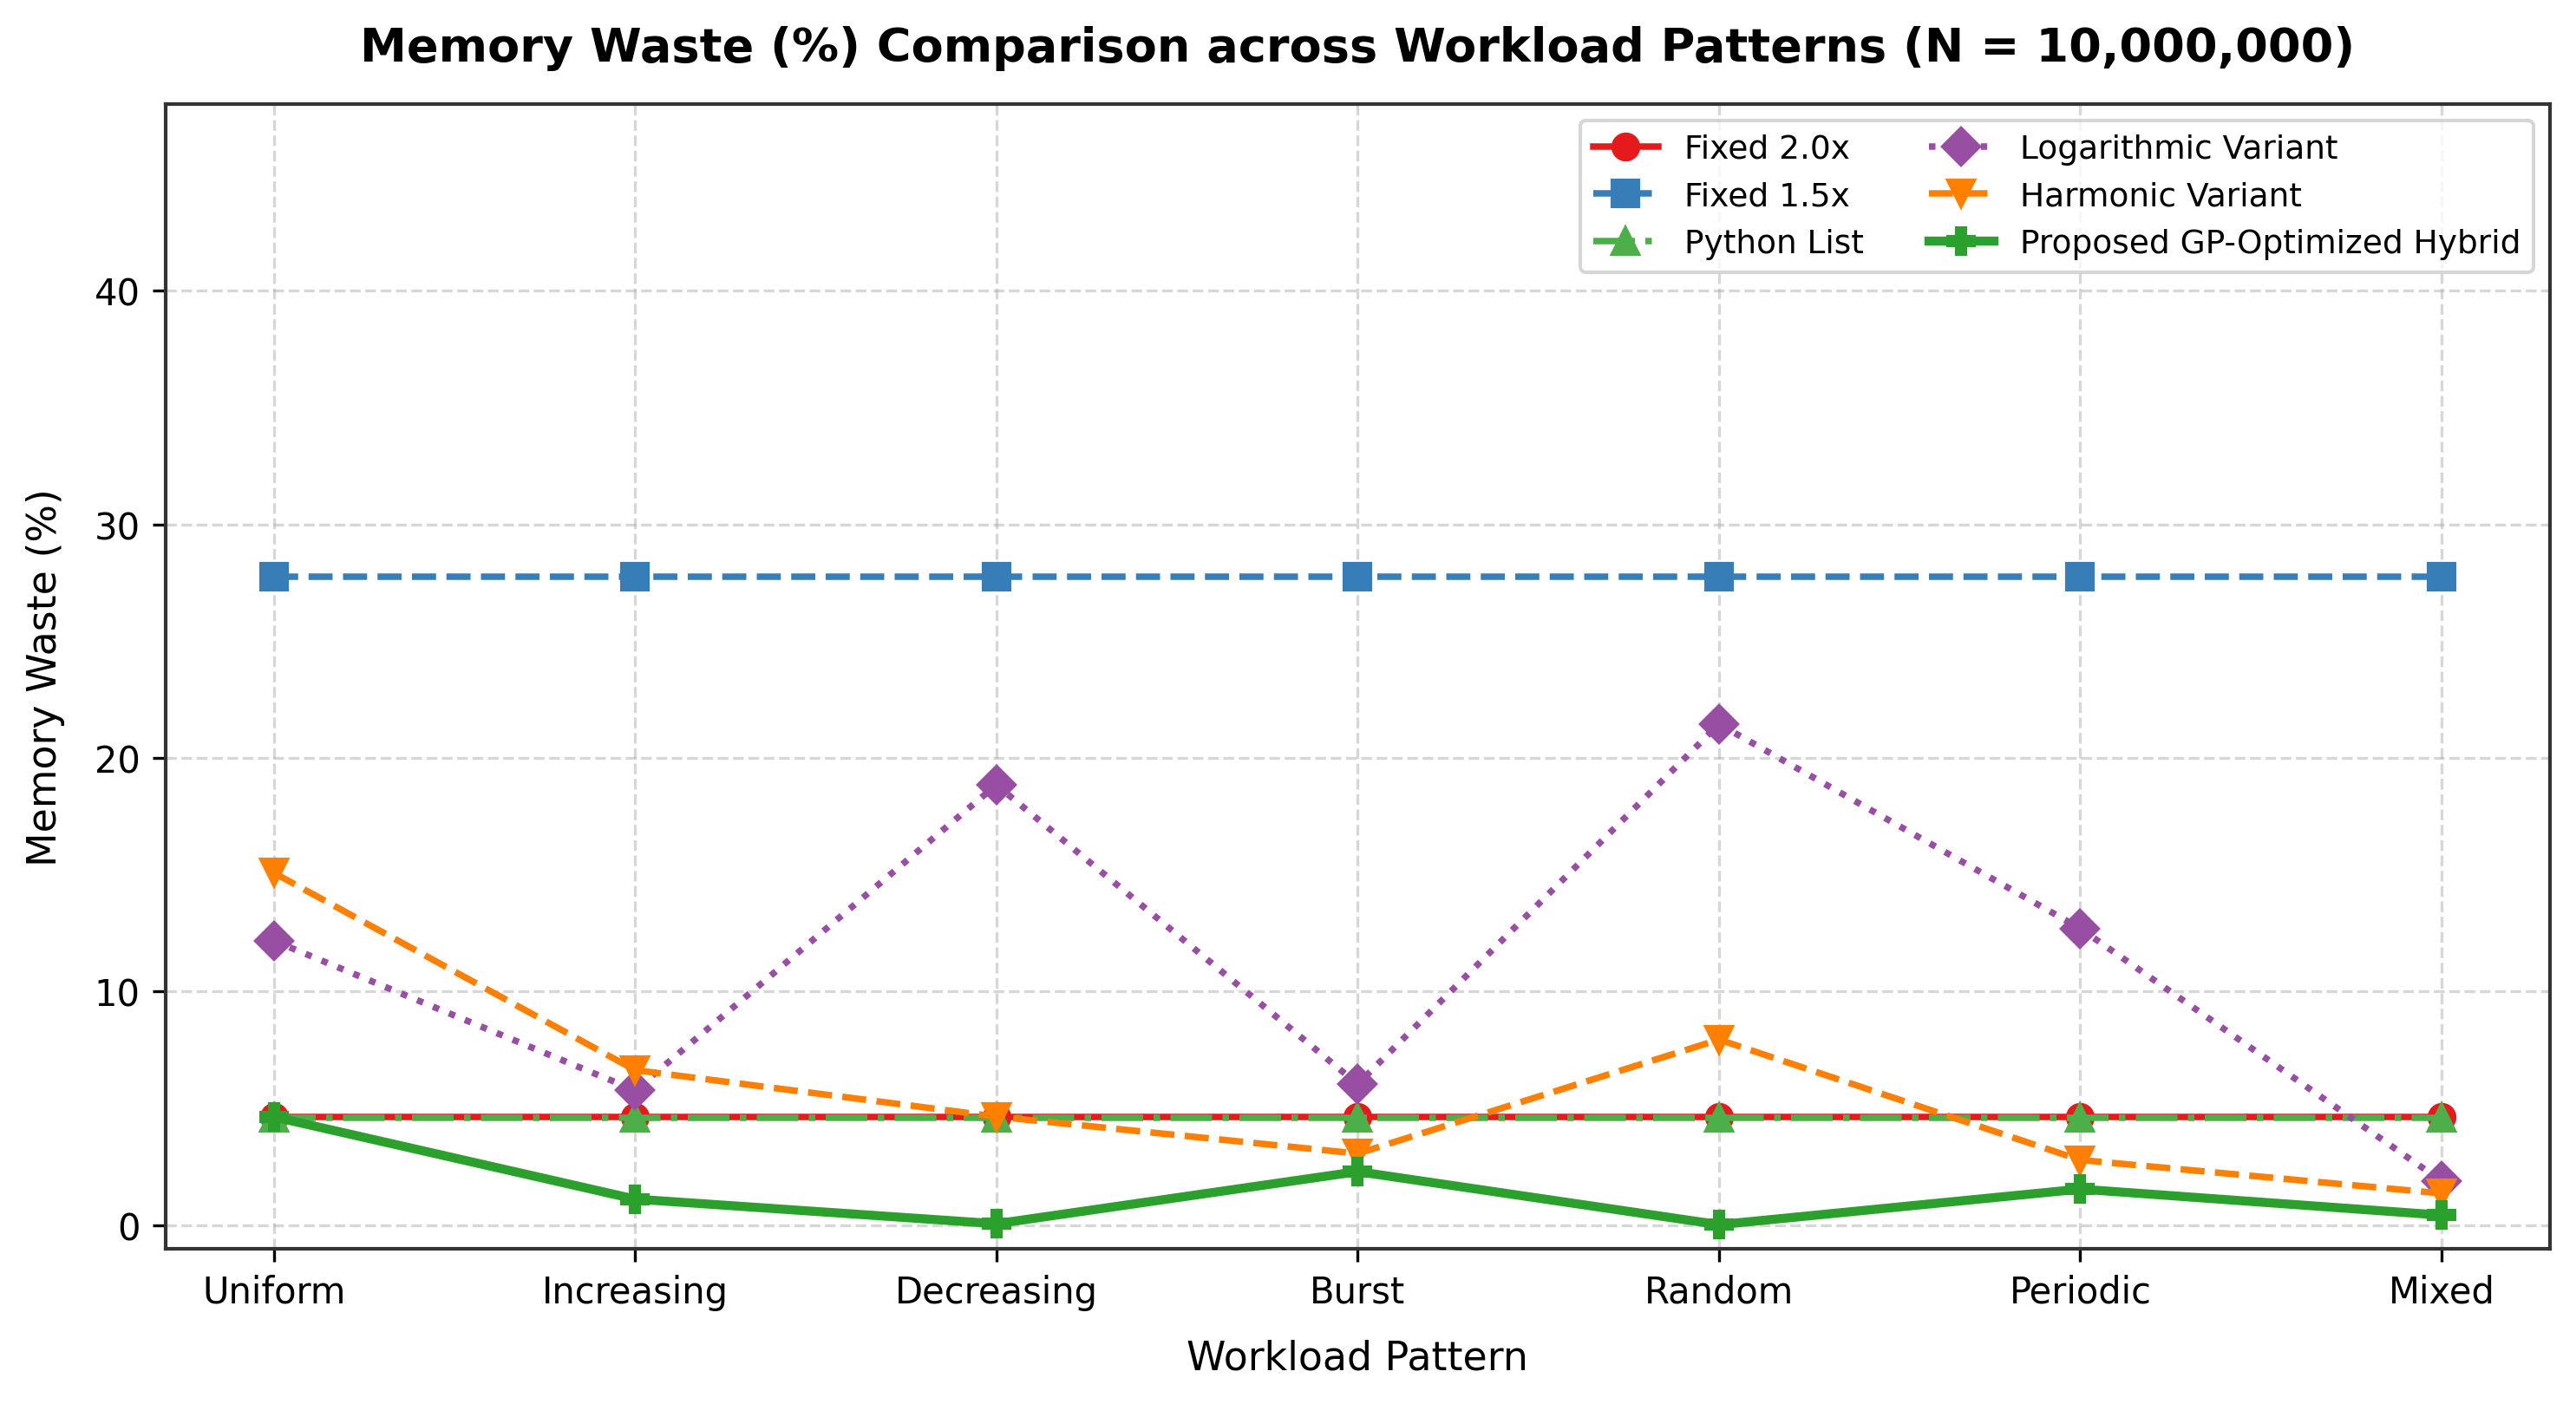
\includegraphics[width=0.75\textwidth]{fd_combined_patterns_line.png}
\caption{Memory waste percentage comparison across seven workload patterns under $10^7$ insertions.}
\label{fig:memory_waste}
\end{figure}

\section*{Keywords}

Dynamic arrays, Adaptive resizing, Workload-aware growth, Memory allocation, Dynamic memory management

\section*{References}

\begin{enumerate}[label={[\arabic*]}]

\bibitem{brodnik}
A. Brodnik, S. Carlsson, E. D. Demaine, J. I. Munro, and R. Sedgewick. \textit{Resizable arrays in optimal time and space}. Technical Report CS-99-09, Department of Computer Science, University of Waterloo, 1999.

\bibitem{sartor}
J. B. Sartor, S. M. Blackburn, D. Frampton, M. Hirzel, and K. S. McKinley. Z-rays: divide arrays and conquer speed and flexibility. \textit{Proceedings of the 31st ACM SIGPLAN Conference on Programming Language Design and Implementation (PLDI)}, 471--482, 2010.

\bibitem{bille}
P. Bille, A. R. Christiansen, M. B. Ettienne, and I. L. Gørtz. Fast dynamic arrays. \textit{Proceedings of the 26th Annual European Symposium on Algorithms (ESA)}, 10:1--10:13, 2018.

\end{enumerate}

\end{document}
